\documentclass{article}
\usepackage{lmodern}
\usepackage{amssymb,amsmath}
\usepackage{longtable}
\usepackage{booktabs}
\usepackage{appendix}
\usepackage{cprotect}

\usepackage{listings}
\lstset{
  numbers=left,
  escapeinside={(*@}{@*)},
  basicstyle=\ttfamily,
  breaklines=true
}
 
\usepackage{comment}
\usepackage{pdfpages}
\usepackage[utf8]{inputenc}
\usepackage[english]{babel}
\usepackage[autostyle]{csquotes}
\usepackage[margin=.5cm]{caption}
% \captionsetup{margin=3cm} inside a figure
% to change only that figure
 
 \usepackage[
 backend=biber,
 style=alphabetic,
 citestyle=authoryear
 ]{biblatex}
% \usepackage[backend=biber]{biblatex-chicago}
\addbibresource{main.bib}


\makeatletter
\DeclareRobustCommand{\KaTeX}{K%
  {%
    \setbox0\hbox{T}%
    \setbox\@tempboxa\hbox{$\m@th$%
      \csname S@\f@size\endcsname
      \fontsize\sf@size\z@
      \math@fontsfalse\selectfont
      A}%
    \@tempdima\ht0
    \advance\@tempdima-\ht\@tempboxa
    \@tempdima\strip@pt\fontdimen1\font\@tempdima
    \advance\@tempdima-.25em
    \kern\@tempdima
    \vbox to\ht0{\box\@tempboxa
      \vss}%
  }%
  \kern-.15em
  \TeX}

\makeatother

\setlength{\parindent}{0em}
\setlength{\parskip}{.5em}
\newcommand{\TeXNet}{Hunter \TeX Net}

\title{\TeXNet{} \textbar{} CSCI 350 Project Proposal}
\author{Alex Taradachuck \and Ralph ``Blake'' Vent\'{e}}
\date{March 2020}

\begin{document}

\maketitle

\begin{abstract}
  The OpenAI request for research spawned research in using Visual Neural Models
  for translating mathematical expressions into markup code. Since the debut,
  progress has been largely incremental. Singh 2018, Wang 2019, and Bender 2019
  all attribute properties of their respect models to the biases in the corpus
  and its pre-processing. We present a new dataset and a pipeline for harvesting
  examples from source files hoping to minimize these biases.
\end{abstract}

\section{Previous Work}

\subsection{Debut}

The prospect of accurately transcribing mathematical expression into a markup
representation is enticing because it opens the doors for bringing new life to
old mathematical texts or those for which the source code is unavailable.

A Harvard project called \emph{What you get is what you see} (\textsc{Wygiwys})
by~\cite{deng2016you} documents strategies for machine translation of
mathematical notation using an attention-based encoder-decoder neural model.
Notably, the researchers were interested in the influence of markup alone on the
efficacy of a model --- without providing explicit information about underlying
grammars \parencite[1]{deng2016you}.

Introduced in 2016 by~\cite{deng2016you}, the \texttt{im2latex100k} dataset has
led research forward by removing the overhead of heavy pre-processing. Using
this dataset, other solutions to \textsc{im2latex} have seen substantial
progress. Recently, it has come under question as a possible \textit{bottleneck} for
progress. We discuss this in greater detail in \ref{datainnov}.

\subsection{Architectural Designs}

Since its inception, solutions to \textsc{im2latex} have used neural models. In
fact, OpenAI's Request for Research recommended the use of a neural model and
even specified the attention machanism that makes these models so powerful, but
there have been a wide variety in the particular architectures of the neural models.

\cite{deng2016you}
\cite{genthial2016image}
\cite{wang2019translating}
\cite{bender2019learning}

\section{Corpus Harvesting}


\subsection{Challenges}

We harvested examples from Cornell's arXiv archive. As the arXiv strictly
forbids scraping, we found a patron who properly obtained copies and uploaded
them to \url{archive.org}. We wrote a script to extract the source code files,
and notably, we use the \texttt{pandoc} document parser.

On this note, \LaTeX{} and its subset, \TeX{} pose an unique set of challenges
compared to other steps of the pre-processing pipeline. \LaTeX{} is a
Turing-Complete language, equivalent in power to general purpose programming
languages. From the theoretical standpoint, it may contain loops and recursion,
classifying it as a recursively enumerable language. As such, no \LaTeX{} parser
is guaranteed to terminate, and regular expressions alone lack the expressive
power to extract all cases of a particular pattern. Practically, we mostly
needed to contend with macro expansion. This means that the original scripts of
\cite{deng2016you} required substantial changes before being suitable for our
purposes.

\subsection{Innovations}
\label{datainnov}

To start, we follow closely in the footsteps of~\cite{singh2018teaching}. After
preprocessing steps on \texttt{im2latex100k}, Singh arrived upon a dataset of
93,784 compiling examples, which he regarded as ``too small for good
generalization.'' As such, he mined additional examples from the KDD Cup 2003
dataset, resulting in about additional 50,000 examples
\parencite[8]{singh2018teaching}.  % also
                                % mention that the others have issues w data[]

Practically, \texttt{pandoc} handled the files from the corpus gracefully, but
due to unlinked files and mismatched encodings, we set \texttt{timeout 5} to
terminate the program after 5 seconds of stalling. \texttt{pandoc} also
facilitates extracting expressions. Without it, we were presented with the
challenging prospect of filtering out text not containing mathematical
% TODO: add example to appendix
expressions, but \texttt{pandoc} generates an abstract syntax tree and encases
the mathematical expressions in the more ``specific'' expression
\verb|\((.*?)\)| compared to the expression \texttt{\$(.*?)\$} which resulted in
false matches that contained only text. One such false match that was eliminated
is provided in the appendix. As a fall-back, we rely on Singh's script to test
for the presence of at least one \LaTeX{} command (from the command vocabulary,
$\Sigma$) before writing out the final formula code. This has the added benefit
of removing examples that are strictly numbers and those that are otherwise
linear strings of alphanumeric characters.
% TODO: cite singh, bender, and wang's objections

Most importantly, \texttt{pandoc} expands all the macros in the source
documents. Without this step, papers in the dataset that relied heavily on
macros to shorten the length of the written expressions contributed very few
formulas to the resulting collection because they caused definition-not-found
errors and were eliminatedin later steps. In~\cite{deng2016you} the processed
formulas were discarded implicitly because they caused such errors, but with the
macros expanding, documents reclaimed their representation in the final set,
eliminating one possible source of bias in the dataset.


%\begin{figure}[!h]
\begin{figure}[]
		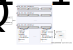
\includegraphics[scale=1.7]{assets/harvest.pdf}
    \centering
    \cprotect\caption{Examples flow from archive.org and are stored on our
    disks, where we extract the \texttt{tar} files first by day, then by
    submission, into the document folders. Then \texttt{pandoc} pulls in all of
    the dependencies of this particular document and writes out one stand-alone
    document with macros expanded. Then we match the regular expression
    \verb|\((.*?)\)| that \texttt{pandoc} uses to wrap mathematical expressions.
    As a general tool \texttt{pandoc} can convert between other markup language
    in the same way, making it useful for standardizing data from disparate
    sources.}\label{datapipeline}
\end{figure}

From~\cite{deng2016you}, we also reiterate that several \LaTeX{} input sequences
map to the same output image, so we use the same normalization with Khan
Academy's \KaTeX{} as they did in their scripts. Like \texttt{pandoc} \KaTeX{}
parses the input sequences into an abstract syntax tree and rebuilds the
expressions without disrupting
semantics. % TODO: everyone got better results with this

\cite[5]{bender2019learning} notes that their \textsc{im2latex} model struggled
very short sequences, and performed better on those that were slightly longer.
They attribute this to an imbalance in the dataset: very short formulas are
underepresented. In fact, this may be traced back to the scripts written by
\cite{deng2016you}, which discarded examples shorter than 40 bytes in length. We
halved the minimum length of an example.

\subsection{Product}

In all, we mined 1 month of \texttt{tar} files, extracted 15,200 \texttt{tex}
files, expanded macros 7,200 unique files and generated data 500,000 rendering
examples. We decided to use about 40\% of that for our final
testing.~\footnote{Data can be found
at~\url{https://github.com/rvente/TeXNet.ai/Dataset .}} A graphical view of our
data pipeline can be seen in Figure~\ref{datapipeline}.

\section{Network Architecture}

Our network has its basis in \citeauthor{singh2018teaching}'s research. The
architecture has several essential features that we enumerate with breif
explanations and proceed with detailed remarks on their implementation in our
architecture.

\begin{description}
  \item[Convolutional Neural Network] Layers in our neural model learn
  convolutions on image space that extracts meaningful information into a
  compressed internal encoding vector.
  \item[Recurrent Neural Network] At time $t$, the network's layer $n$ takes as
  input the output of layer $n$ at time $t-1$. To train such a network using
  backpropagation, it is "unrolled" so as to emulate a feed-forward network,
  allowing the updates to propagate.
  \item[Long-Short Term Memory] Looseley speaking, the LSTM cells in the neural
  network "learn when to forget" about a particular subset of the previous
  layer's output. This allows for reasoning over time.
\end{description}

\section{Evaluation}

For evaluation, we use Bilingual Evaluation Understudy (BLEU), the emerging
standard among neural network solutions to the \textsc{im2latex} problem. BLEU
is an automated metric for assessing machine translation accuracy
\cite[1]{papineni2002bleu}. 

\printbibliography{}

\begin{appendix}
  \section{Lessons Learned in Data Cleaning}
\begin{figure}[]
  \begin{lstlisting}[escapechar=!, basicstyle=\small\ttfamily, firstnumber=1132]
    The net flow vector $(1,1,0,\hdots,0)$ has previously been considered for the complete graph by Corteel, Kim, and M\'esz\'aros \cite{CKM}.  They used the Lidskii formula~\eqref{eq:lidskiivol} and constant term identities to derive the following product formula for the volume of $\mathcal{F}_{K_{n+1}}(1,1,0,\ldot     s,0)$.
    It would be of interest to rederive this result using the refined Kostant constants.
   \begin{theorem}[{\cite[Theorem 1.1]{CKM}}] \label{thm:volkn11}
   Let $n\geq 1$. For the complete graph $K_{n+1}$,

  \end{lstlisting}
  \begin{lstlisting}[basicstyle=\small\ttfamily]
  s,0)$. It would be of interest to rederive this result using the refined Kostant constants. \begin{theorem}[{\cite[Theorem 1.1]{CKM}}] \label{thm:volkn11} Let $    
  \end{lstlisting}
   \cprotect\caption{Math encased in dollar-signs has been deprecated in
  \LaTeX{}, but remains in wide use as an artifact from \TeX{}. It was
  deprecated to facilitate parsing: unlike \verb|\(| which indicates that it
  opens to the right, the dollar-sign has no such indication. The reason the
  previous scripts were matching text was because the hanging \verb|$| of the
  first line matched with the very first dollar sign of the 4th line. Viewed another way,
  the regex was using the same token twice, which initially caused a false match marked as (1).
}


\end{figure}

\end{appendix}
\end{document}
